\chapter{Background}\label{chap:background}
At a high level, the production of dairy farming and livestock can be expressed as the result of a phenotype product $P$ which is a combination of a genotype $G$ realization and environmental factors $E$: $P = G + E + G \times E$ \citep{adhikari_climate_2022}. The genetic factors $G$ are influenced by breeding. The environmental factors $E$ are farm management practices such as housing or feeding, policy and socio-economic environment, ambient weather and climate. Both breeding strategies and changing environmental conditions impact susceptibility to heat stress, dairy performance, animal health and reproduction. The interaction between the G and E determines to which degree a dairy cow may express the full genetic potential with respect to a selected metric such as milk performance.

\vspace*{\baselineskip}
Given the animal-level nature of our dataset, this chapter starts with an overview of the physiological aspects of dairy cows under heat stress conditions in Section~\ref{sec:animal_physiology}. We thereby highlight critical factors that may necessitate modelling. Then, in Section~\ref{sec:breed_models} we analyze a range of selected models estimating heat-effects across breeds to appraise the current technical state-of-the art and identify potential gaps. This is followed by a comprehensive review of the developments in Swiss milk production over the past four decades in Section~\ref{sec:evolution_market}, aligning with the scope of our data: breeding associations set long-term goals which ideally increase the milk yield in the long run. Moreover, legislative amendments and policy measures can substantially influence farm management practices and breeding techniques. Collectively, this chapter establishes the foundational understanding of factors that may inform the modeling process in Chapter~\ref{chap:material_methods}.

\newpage

\section{Animal Physiology}\label{sec:animal_physiology}
This section summarizes key concepts in animal physiology pertaining to heat stress. Unless explicitly indicated otherwise, the review from \cite{kadzere_heat_2002} serves as the source of information for this section and its subsequent subsections. We discuss some aspects of the cow physiology to better understand the complex heat-related interactions between the animal $G$ and the environment $E$. Moreover, the section highlights physiological arguments, why we might expect different heat stress responses for different breeds.


\begin{figure}[ht]
    \centering
    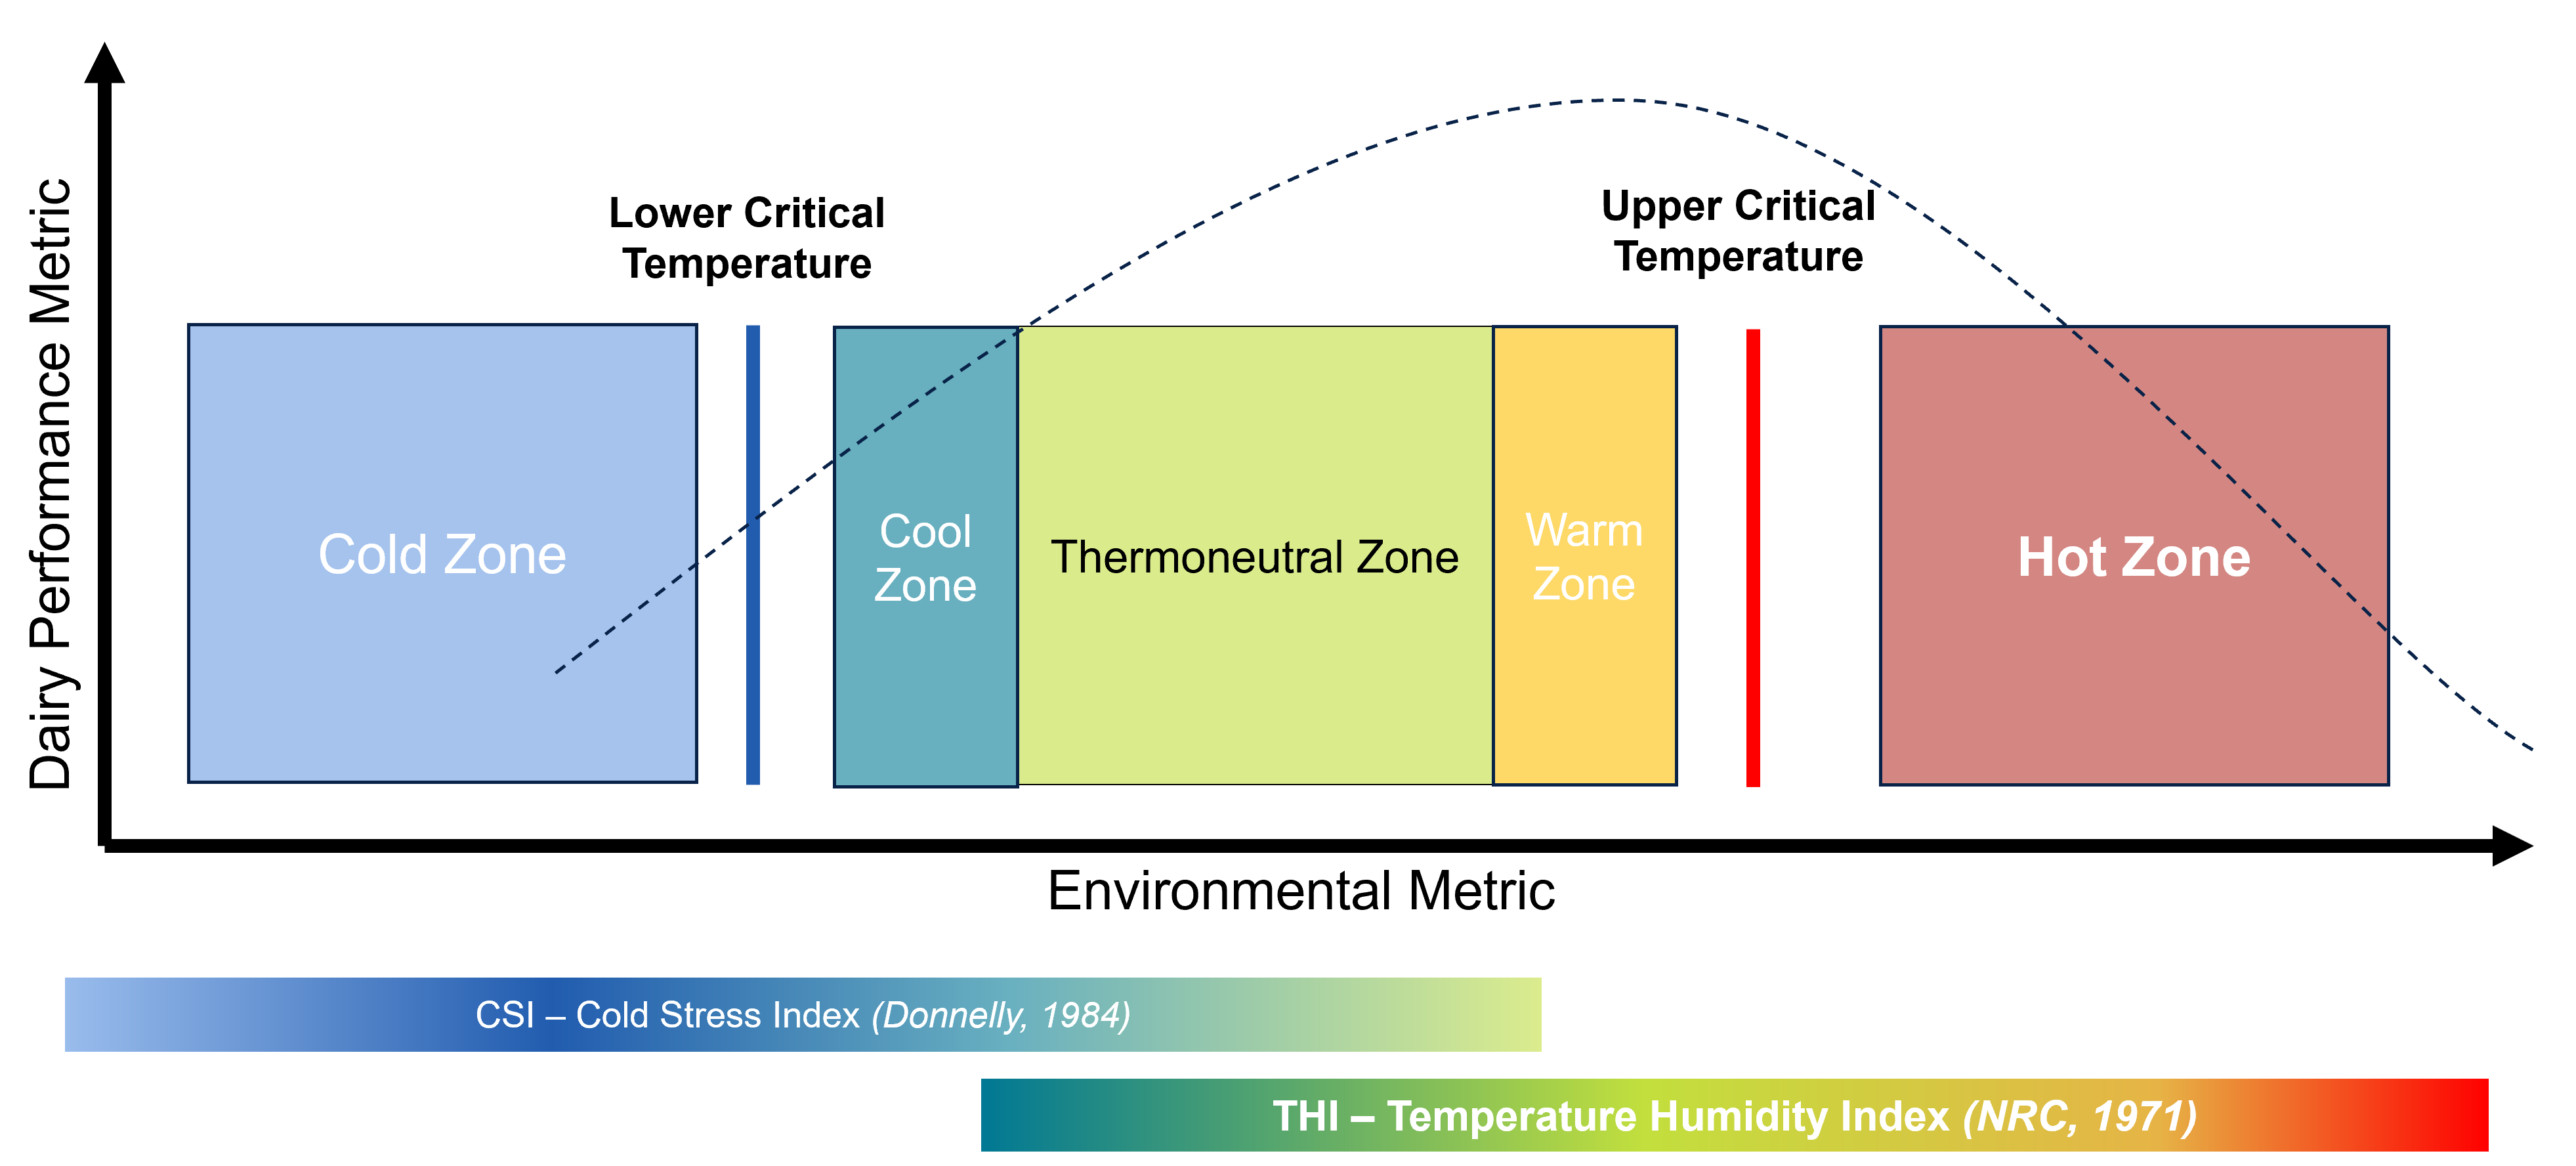
\includegraphics[width=\textwidth]{thesis/figures/physiology.png}
    \caption{Animal physiology: a dairy cow achieves maximum productivity at minimal physiological costs in the thermoneutral zone. A broadly accepted environmental metric to measure heat stress is the Temperature Humidity Index (THI).}
    \label{fig:ainmal_physiology}
\end{figure}

\vspace*{\baselineskip}
\begin{defi} Heat Stress in Dairy Cows \\
    Heat stress is the collective impact of high temperatures compelling adjustments from sub-cellular to the whole animal level in order to avoid a physiological dysfunction and adapt better to the current environment. 
\end{defi}

As a homothermal the cow must maintain a thermal equilibrium with the environment to regulate the biochemical reactions and physiological processes. The environmental factors include air temperature, air movement, humidity, as well as radiation. When cows fail to balance their body temperature within their thermoneutral zone and keep it in physiological homeostasis, they will experience hyperthermia, which may lead to death. The main characteristics of heat stress, independent of any effects of feed intake, are elevated respiration rates, increased rectal temperatures, an impaired metabolism, reduced growth and lactation, as well as poor reproductive performance.

\subsection{Thermoregulation}\label{sec:thermoregulation}
\paragraph{Heat Increment}
The heat production in the dairy cow serves to maintain equilibrium with heat dissipation mechanisms and is controlled by the nervous system, endocrine system, appetite, digestion, respiratory enzymes as well as protein synthesis. Factors affecting the heat production intensity are the ambient temperature, hormone concentrations such as growth hormones, body size, breed, fodder and water availability. Heat increment is the increase in body heat production resulting from digestation, heat absorption and the metabolism of nutrients activated through feed intake. Large amount of feed intake generate significant metabolic heat. Moreover, an increased milk production relates to a raised heat increment. The heat increment during the lactogenesis depends on the fodder quality and quantity. The milk production capacity also depends on the cow size. The latter is linked to the size of their gastrointestinal tracts, which have bigger digestion capacity in larger cows. This increased capacity results in a higher substrate availability for the milk production. 

\paragraph{Heat Dissipation}
Dairy cows lose heat through factors such as sweating, changes in environmental temperature, changes in the radiating surface, air flow changes, or convection. The amount of radiant heat a cow absorbs is influenced by the environmental temperature and its coat color. Dark-coated cows, for instance, generally absorb more heat than those with lighter brown coats. Cows can release metabolic heat through evaporative cooling, wherein water absorbs heat from the cow's surface. The degree of heat loss through evaporation rises with increasing ambient temperatures. Additionally, convection serves as a method for heat dissipation when cooler air circulates around the warmer body, absorbing heat which is then carried away. However, if the surrounding air is warmer than the cow's skin, heat is instead transferred into the animal's body. Conductive transfer, another form of heat exchange, happens when the cow is in direct contact with another surface or entity. Unlike convection, which entails the movement of the subject, conduction involves heat transfer without the displacement of the subject. Conduction becomes pertinent when a cow is lying down, thus selecting appropriate ground surfaces or bedding materials is important for both animal welfare and strategies to mitigate heat stress.

\paragraph{Thermoneutrality}
Overall, the maintenance of thermoneutrality requires an equilibrium between heat gains and heat losses with the environment. This can be stated with the following heat balance equation $M = \pm K \pm C \pm R + EV$, where $M$ is the metabolic heat production, $K$ is the heat exchanged by conduction, $C$ by convection, $R$ by radiation, and $EV$ by evaporation. Generally, the thermoregulatory response of dairy cows may have changed over time since breeding strategies promote a genetic selection for an increased milk production (c.f. Figure~\ref{fig:dataset_structure_time_seasonality}).

\paragraph{Heat Stress}
When a cow absorbs more heat than it can dissipate, it experiences heat stress. Factors such as environmental conditions and specific animal traits such as age, breed, sex, metabolic state, coat condition, nutrition, and health status contribute to heat stress. For instance, Jersey and Holstein cows have varying rates of heat production and dissipation, which could be attributed to differences in body size. Additionally, performance indicators such as productivity, growth, and fertility are other factors influencing heat stress. These aspects are also affected by the type of housing, geographic location, the efficiency of ventilation systems, and the cow's social rank within the herd. Generally, high-producing dairy cows are more affected because the thermoneutral zone shifts to a lower temperature range with a higher milk production, feed intake and metabolic heat production \citep{gantner_differences_2017, tapki_comparison_2006}.

\paragraph{Regulation Mechanism}
Within the thermoneutral zone (TNZ), heat production is kept to a minimum under typical body temperatures, ensuring optimal physiological performance and maximum productivity. The lower limit of the TNZ is known as the lower critical temperature (LCT) and the upper limit as the upper critical temperature (UCT). For dairy cows, the TNZ spans about 5-25°C, with an UCT ranging from approximately 25-26°C \citep{becker_invited_2020}. If the surrounding temperature falls below the LCT, the cow must elevate its heat production to maintain thermal balance. Between the LCT and UCT, the cow sustains its body temperature. An example reported LCT range is -17° to-30°C \citep{kadzere_heat_2002, bryant_quantifying_2007}. However, as the ambient temperature rises within the TNZ, evaporative heat loss diminishes, which is counteracted by vasodilation and increased water evaporation. Upon reaching the UCT, heat production rises due to inadequate evaporative cooling. When thermal stress exceeds the evaporative loss capacity, the cow may enter a state of hyperthermia. The specific values for LCT and UCT are influenced by factors such as age, species, breed, feed intake, diet composition, tissue and external insulation, as well as animal behavior. Figure~\ref{fig:ainmal_physiology} depicts the interplay between the different thresholds.

\paragraph{Heat Stress Response}
Thermal sweating is a common response to heat stress. It plays a role in evaporative cooling and occurs when ambient temperatures rise, reducing the temperature gradient with the animal's body. An increase in sweating is positively correlated with enhanced blood flow to the cow’s skin, and sweat rates can vary among different breeds. Breed variations influence how respiration rates respond to elevated temperatures; for example, Jersey cows often display higher respiration rates compared to Holsteins, suggesting better heat dissipation in Holsteins. Rising relative humidity during heat stress can result in decreased respiration rates, increased surface evaporation, raised rectal temperatures, reduced feed intake, and diminished milk production. Short-term heat exposure reduces heart rate as a stress response, though this effect diminishes with long-term exposure. Dairy cows under heat stress show reduced growth hormone levels because metabolic heat production must be lowered. High temperatures may enhance digestive efficiency due to prolonged feed retention and decreased dry matter intake. To manage heat stress, dairy farmers employ protective measures, breeding strategies, and dietary adjustments. Quantifying the direct impact of environmental conditions on milk production is complex due to intricate interdependencies such as farm management. Nonetheless, research consistently shows a negative relationship between heat stress and milk output, including volume, fat, and protein content. Table~\ref{table:heat_stress_expected_effects} lists the expected effects on selected dairy performance metrics for lactating dairy cows.

\begin{table}[H]
    \centering
    \begin{tabular}{lll}
    \textbf{Variable} & \textbf{Effect} & \textbf{References} \\
    \midrule
    \midrule
    Milk & Decrease & \cite{ahmed_temperature_2022, gisbert-queral_climate_2021} \\
    \hline
    Fat & \multrow{no effect$^*$ \\ decrease$^\dag$} &  \cite{vroege_effects_2023}$^*$, \cite{moore_how_2023}$^\dag$,\cite{ vinet_estimation_2023}$^\dag$\\
    \hline
    Protein & Decrease & \cite{gao_effects_2017, vinet_estimation_2023} \\
    \hline
    \hline
    SCC & Increase & \cite{hammami_evaluation_2013,lievaart_effect_2007} \\
    \hline
    MUN & Increase & \cite{gao_effects_2017} \\
    \hline
    BHB & Increase & \cite{stefanska_effect_2024} \\
    \hline
    Lactose & \multrow{no effect$^*$ \\ Increase$^\dag$} & \cite{kadzere_heat_2002}$^*$, \cite{moore_how_2023}$^\dag$\\
    \hline
    Citrate & Increase & \cite{tian_integrated_2016} \\
    \hline
    Aceton & Increase & \cite{tian_integrated_2016} \\
    \bottomrule
    \end{tabular}
    \caption{Expected impact of heat stress on dairy performance performance: milk, fat protein are the primary variables of interest for our study. Somatic cell count (SCC), milk urea nitrogren (MUN), $\beta$-hydroxybutyrate (BHB), lactose, citrate and aceton are provided for complementary purposes.}
    \label{table:heat_stress_expected_effects}
\end{table}

\paragraph{Adaptation}
Dairy cows, akin to other homeothermic animals, have physiological processes to maintain their body temperature over a spectrum of environmental temperatures. The capacity to adapt to changing environmental conditions differs among species and breeds. For example, in an experiment with high-yielding cows which perform best in temperate climates, relocating them to tropical areas leads to reduced milk yield. Breeds that are native to tropical climates exhibit unique traits like decreased feed consumption, lower metabolism, improved heat release due to greater body surface areas, and either more sweat glands or shorter hair, assisting in transferring heat from the body's center to the skin and environment. Research on heat stress indicates that Holsteins show more significant drops in milk and protein output than Jerseys under such conditions. The effects of adaptation diminish when exposure to heat stress lasts for several weeks. Moreover, dairy cows show a dual-phase daily cycle, with rising body temperatures from midnight to early morning and again from afternoon to evening. Lowering nighttime temperatures can counteract high daytime temperatures, offering some protection \citep{araki_diurnal_1987}. However, this protection is lost if nighttime temperatures remain elevated. Typically, these adaptation mechanisms can sustain regular productivity in warm climates. Even high-milk-producing cows can adapt during warm summer periods as they slowly acclimate to warmer weather. Nonetheless, sudden and extended extreme heat reduces the likelihood of adaptation and heightens the exposure to heat stress\citep{vroege_effects_2023}. 


\subsection{Temperature Humidity Index}
The Temperature Humidity Index (THI) is a metric to indicate the thermal climatic conditions with temperature and relative humidity. It is used as a proxy for heat stress levels and exposure as depicted in Figure~\ref{sec:animal_physiology} with the goal to give a more precise measure of environmental stress on cows than a single variable. The THI is a simple, comprehensive measure and used as a tool for productivity insights, farm management decisions such as cooling systems or fodder adjustments, and animal welfare. The simplicity of the measure might be a reason for the wide acceptance in academia and industry. Disadvantages of the THI are the limitation to two variables whereas other environmental variables such as radiation, wind speed, precipitation also affect the thermal balance of dairy cows as discussed in Section~\ref{sec:thermoregulation}. Moreover, THI is not standardized \citep{moore_how_2023}. Oftentimes, the THI is used with threshold values to decide if a cow is exposed to heat stress or not. However, these may not globally apply and depend on the location and other factors such as the cow breed. Each individual animal may have varying heat stress tolerances. Different THI formulas for different regions are available to accommodate climate and environmental heterogeneity \citep{bohmanova_temperature-humidity_2007}. For the remainder of this work we use the THI definition from the \cite{nrc_1971}:
\begin{defi} Temperature Humidity Index (THI)
\begin{equation}
    \text{THI} = (1.8 \times \text{T}) + 32 - \left[ (0.55 - 0.0055 \times \text{RH}) \times (1.8 \times \text{T} - 26) \right],
\end{equation}
\end{defi}
where $T$ is the air temperature in [°C] and $RH$ the relative humidity in [\%].  Figure~\ref{fig:thi_table} provides a THI mapping of the temperature from 0-40°C and the relative humidity from 0-100\%.

\section{Modelling Heat Stress Across Breeds}\label{sec:breed_models}
The preceding Section~\ref{sec:animal_physiology} discusses the manner in which diverse physiological characteristics, potentially unique to specific dairy cow breeds, influence their responses to heat stress. We have only identified three studies that explore the impact of weather conditions on dairy cow breeds within commercial pasture-based agricultural systems. Table~\ref{table:breed_study_comparison} provides a brief comparison between their and our work. The subsequent subsection will provide brief summarizes of their methodology.

\begin{table}[H]
    \centering
    \begin{tabular}{ccrrrcc}
        \textbf{Study} & \textbf{Breeds} & \textbf{Records} & \textbf{Farms} & \textbf{Cows} & \textbf{Time} & \textbf{Location} \\
        \hline
        \hline
        \multrow{\citeauthor{bryant_quantifying_2007} \\ \citeyear{bryant_quantifying_2007}} & \multrow{Holstein \\ NZ Jersey \\ HF/NZJ} & 65'905 & 496 & 19'201 & 1990-2002 & New Zealand \\
        \hline
        \multrow{\citeauthor{gantner_differences_2017} \\ \citeyear{gantner_differences_2017}} & \multrow{Holstein \\ Simmental} & \multrow{1'070'554 \\ 1'300'683} & \multrow{5679 \\ 8827} & \multrow{70'135 \\ 86'013} & 2005-2012 & Croatia \\
        \hline
        \multrow{\citeauthor{ahmed_temperature_2022} \\ \citeyear{ahmed_temperature_2022}} & \multrow{SE Holstein \\ SE Red \\ SH/SRB \\ Other} & \multrow{2’893’367 \\ 1’279’758 \\ 417’312 \\ 973’729} & 1'435 & ? & 2016-2019 & Sweden \\
        \hline
        \multrow{Our work \\ 2024} & \multrow{Holstein \\ Brown Swiss \\ Original Braunvieh \\ Simmental \\ Swiss Fleckvieh \\ Jersey} & \multrow{27'536'089 \\ 56'695'597 \\4'996'060 \\ 8'731'876 \\ 31'484'784 \\ 734'685} & \multrow{24'963 \\ 26'585 \\ 18'613 \\ 19'411 \\ 27'392 \\ 4'302} & \multrow{971'198 \\ 1'719'156 \\ 149'478 \\ 299'698 \\ 1'038'291 \\ 23'675 } & \multrow{1985-2023 \\ 1982-2023 \\ 1982-2023 \\ 1984-2023 \\ 1984-2023 \\ 1998-2023} & Switzerland \\
        \hline
        \end{tabular}\label{table:study_comparison}
        \caption{Comparison of studies analyzing heat stress across breeds with production farm data.}
        \label{table:breed_study_comparison}
\end{table}

\subsection{Cow-Level Milk Yields Across Breeds (New Zealand)}\label{sec:new_zealand}
\cite{bryant_quantifying_2007} propose a mixed-model to quantify effects of the thermal environment across three breeds in New Zealand. Their focus is on heat stress as well as cold stress. Hence, they work with two environmental indexes THI and cold stress index CSI as depicted in Figure~\ref{fig:ainmal_physiology}. The study utilizes data provided by a corporation managing over 400 herds distributed across various regions of New Zealand. The sample set is restricted to first lactation spring-calving animals exclusively. Let $\mathcal{H}$ denote the set of individual herds or farms, $\mathcal{Y}$ the years for which data is available, $\mathcal{B}$ the breeds under examination, and $\mathcal{D}$ the test days considered. The dependent variables employed in this analysis include daily milk yield, as well as daily fat and protein concentrations. The model is defined as

\begin{defi} Heat Stress Model by \cite{bryant_quantifying_2007}
    \begin{equation}
    y_{i,j,k,l} = \mu + H_i + Y_j + B_k + b_1 a_{i,j,k} + b_2 d_{i,j,k} + \sum_{n=0}^{4} \alpha_n P_n(t_{i,j,k,l}) + \sum_{o=1}^2 \gamma_o x_{i,j,l} \times B_k + x_{i,j,k}^o + \epsilon_{i,j,k,l},
\end{equation}
\end{defi}
 where $H_i$ is the fixed class effect for herd $i \in \mathcal{H}$, $Y_j$ the fixed class effect for year $j \in \mathcal{Y}$, $B_k$ the fixed class effect for breed $k \in \mathcal{B}$, $a_{i,j,k}$ the age of the cow at calving in months, $d_{i,j,k}$ the parturition date deviation from the heard-year parturition date, $t_{i,j,k,l}$ the days in milk for test day $t$, $x_{i,j,l}$ the 3-day average of the environmental index, $c_{i,j,k}$ the annual random permanent effect of cows in herd $i$\footnote{It remains unclear if this a factor level per animal or not.} and year $j$ for the breed $k$, and $\epsilon_{i,j,k,l}$ is the error term. Accordingly, $b_1$ and $b_2$ are the age and parturition coefficients, $\alpha_n$ are the Legendre polynomial coefficients measure time effects with respect to days in milk, and $\gamma_o$ measure the effect of the environmental index separately for each breed.

\paragraph*{Limitations} The effect of THI and CSI is modelled as an inverse parabola and poses therefore some preliminary assumption about the non-linear effect of THI. 


\subsection{Cow-Level Milk Yields Across Breeds (Croatia)}\label{sec:croatia}
\cite{gantner_differences_2017} analyze the impact of the THI to the daily milk yield and the somatic cell count in Croatia with a mixed model approach. Both breeds are split into a high and low production level in terms of their daily milk yield. A fixed-effect regression is executed on each combination of integer THI values, breed and production level. The effects days in milk, calving seasons, age at calving, region and a binary heat stress indicator. To evaluate, the authors compute the difference on the mean square scores for each THI category and test for significance with Scheffe's method.
\paragraph*{Limitations} The method does not take into account the non-linear effects of the THI on dairy cows. The authors use a mixed-model, but do not declare random effects. Moreover, critical THI levels are assumed to be in a range between 68 and 78.

\subsection{Farm-Level and Cow-Level Milk Yields Across Breeds (Sweden)}\label{sec:sweden}
\cite{ahmed_temperature_2022} employ several modelling approaches. One approach assesses the impact of temperature on average dairy production at the farm level, incorporating temperature as a non-linear smooth function. This methodology is considered more robust than the methods described in Section~\ref{sec:new_zealand} and Section~\ref{sec:croatia} since it allows for unrestricted non-linear temperature effects. The second approach utilizes a linear model with animal-level data to determine whether diversifying a herd with different breeds can serve as a strategy for mitigating heat stress.

\subsubsection*{Milk Performance Estimation}
The authors use Generalized Additive Models (GAMs) to estimate the relationship between weather and milk performance variables. The dependent variables are the average milk produced per cow [kg/day], average energy-corrected milk (ECM) produced per cow [kg/day] and bulk milk somatic cell counts (BMSCC) [cells/ml]. As above, the set $\mathcal{I}$ defines the farms. The measurement periods are set as years in $\mathcal{T}$. The seasons within a year are defined in $\mathcal{S} =$ \{Winter (December-Februrary), Spring (March to May), Summer (June to August), Automn (September to November)\}. The penalized spline regression is

\begin{defi} Temperature Effect on Dairy Performance by \cite{ahmed_temperature_2022}
\begin{equation}\label{method:ahmed_1}
    \textit{Milk}_{i,s,t} = \beta_0 + \sum_{j=1}^{p} f_i[(\textit{Temp}_{i,s,t})] + \gamma X_{i,s,t} + \mu_{i,s} + \epsilon_{i,s,t}\quad,
\end{equation} 
\end{defi}

where $i \in \mathcal{I}$,  $t \in \mathcal{T}$ and $s \in \mathcal{S}$. Confounding effects of humidity and precipitation on temperature are controlled by $X_{i,s,t}$ which is the sum of their first and second order terms. $\mu_{i,s}$ controls for unobserved farm characteristics and farm-specific seasonality. $\epsilon_{i,s,t}$ is the error-term. $f_j$ are the non-parametric polynomial smooth functions for which the number of functions $p$ and spline coefficients are estimated with a penalized log-likelihood method.

\subsubsection*{Breed Diversification}
Moreover, the authors aim to validate breed diversification as a heat stress adaptation measure. In this case the available farms are defined in $\mathcal{J}$ and the cows in $\mathcal{I}$. Let $\textit{Hw}_{j,s,t}$ be a heatwave indicator variable $\mathbbm{1}\left (\bigwedge_{\tau=t-\delta}^{t} (\textit{Temp}_{j,\tau} \geq T)\right )$ which equals 1 if the temperature on farm $i$ has been over a threshold $T$ during the last $\delta$ days. They set $\delta=6$ to cover the past week of the milk recording day and the maximum temperature $T=25$°C. The set $\mathcal{M}=\{$SH, SRB, SH/SRB, Others$\}$ represents the available breeds, where SH is Swedish Holstein, SRB Swedish Red and SH/SRB a mixed breed. The variable $\textit{Breed}_{m,i}$ be the indicator variable $\mathbbm{1}\left (\textit{Breed} = m \right )$ assigning the breed $m \in \mathcal{M}$ to cow~$i$. $X_{i,j,s,t}$ summarizes the first and second order farm-level humidity and precipitation, as well as the days in milk and the lactation number of a cow $i$. The following regression incorporates the breeds

\begin{defi} Breed Diversification by \cite{ahmed_temperature_2022}
    \begin{equation}
    \textit{Milk}_{i,j,s,t} = \alpha_0 + \phi \textit{Hw}_{j,s,t} + \sum_{m \in \mathcal{M}} \alpha_m \textit{Breed}_{m,i} + \sum_{m \in \mathcal{M}} \delta_m \textit{Breed}_{m,i} \times \textit{Hw}_{j,s,t} +  \rho X_{i,j,s,t} + \theta_{j,s} + \epsilon_{i,s,t}\quad ,
\end{equation}
\end{defi}

 where $i \in \mathcal{I}$, $j \in \mathcal{J}$, $t \in \mathcal{T}$ and $s \in \mathcal{S}$. $\alpha_m$~captures the effect on milk production of each breed $m$. $\delta_m$~reflects the effect of the breed on milk production during a heatwave. $\theta_{j,s}$~are the farm-level seasonal fixed effects. $X_{i,s,s,t}$ are farm-level weather controls as well as cow control variables such as days in milk and parity.

\section{Evolution of the Swiss Dairy Market}\label{sec:evolution_market}
Our study encompasses a time period from 1982 to 2023. Switzerland's dairy industry is a structured and regulated market, which currently constitutes the most significant sector of Swiss agriculture. This section focuses on the evolution of the Swiss dairy market in the past 40 years. We focus on policy interventions that affect dairy cow husbandry and, consequently, have implications for milk production. The policy interventions are summarized in Table~\ref{table:policies}.

\begin{table}[H]
\centering
\begin{tabular}{p{4cm}p{5cm}m{2cm}m{2cm}c}
    \textbf{Policy} & \textbf{Description} & \textbf{Enactment} & \textbf{Expiration}\\
    \hline
    \hline
    Milk quotas & limit producion, penalize excess & 1977 & 2009 \\
    \hline
    RAUS & free-range production system & 1993 & -\\
    \hline
    BTS & free-stall barns & 1996 & -\\
    \hline
    Milk price supplement & cheese production, silage-free milk & 1999 & -\\
    \hline
    Grassland-based feeding & less concentrate & 2014 & -\\
    \hline
    Commercial milk & export loss compensation & 2019 & -\\
    \hline
    Pasture payment & ample outdoor access & 2023 & -\\
    \hline
    Cow longevity & optimize longevity  & 2024 & -\\
    \end{tabular}
    \caption{Policies tangential to Swiss milk production.}
    \label{table:policies}
\end{table}

\paragraph{1950-1990: Protective Years}
In the period following World War II, although a liberal economic policy predominantly prevails, the Swiss agricultural sector is characterized by the implementation of price guarantees, sales commitments, and tariffs, notably within the domain of dairy production \citep{huber_lessons_2023}. The agricultural act of 1951 ensures prices for agricultural commodities that cover production costs. Concurrently, milk production undergoes economic rationalization, marked by a reduction in the number of producers juxtaposed with an increase in the volume of milk production. Enhanced dairy productivity leads to subsidies covering production costs rising to an annual level of CHF $0.5$ billion in the 1970s. To mitigate the expansion of dairy production, farm-level milk production quotas are introduced in 1977, based on factors such as the area of agricultural land and the farm's geographical location. \citep{huber_lessons_2023}. Collectively, dairy production accounts for up to 54\% of federal agricultural subsidies \citep{milchwirtschaft_2015}. This system results in production surpluses which are then sold on international markets, thereby imposing significant financial obligations on the federal government to support producer prices. Additionally, the intensive production system prompts environmental concerns \citep{huber_lessons_2023}.

\paragraph*{1990-2010: Decoupling and Liberalization}
In 1992, as a consequence of the previously mentioned national agricultural challenges and external pressure to comply with international standards, decoupled direct payments are instituted to support farmers independently of their production output and location, thus ensuring the maintenance of social and environmental standards. These direct payments comprise lump-sum area payments and ecological payments. The RAUS\footnote{\href{https://www.blw.admin.ch/blw/de/home/instrumente/direktzahlungen/produktionssystembeitraege23/tierwohlbeitraege1.html}{Regemässiger Auslauf ins Freie}} program is introduced in 1993 to encourage free-range production systems. The program mandates that dairy cows have access to pasture during the summer and to uncovered outdoor areas during the winter. In 1996, the BTS\footnote{\href{https://www.blw.admin.ch/blw/de/home/instrumente/direktzahlungen/produktionssystembeitraege23/tierwohlbeitraege1.html}{Besonderns tierfreundliche Stallhaltungssysteme}} program is inaugurated, promoting animal-friendly housing systems such as free-stall barns. This action-based payment scheme is calculated annually per livestock unit, providing compensation for additional investment and workload.

A significant policy reform in 1999 links the eligibility for direct payments to the adherence to cross-compliance standards\footnote{\href{https://www.blw.admin.ch/blw/de/home/instrumente/direktzahlungen/oekologischer-leistungsnachweis.html}{Ökologischer Leistungsnachweis}}. Furthermore, in 1999, price support measures for milk are abolished and tariffs are reduced to comply with international agreements. Concurrently, a milk price supplement payment for dairy milk processed into cheese and silage-free milk\footnote{\href{https://www.blw.admin.ch/blw/de/home/nachhaltige-produktion/tierische-produktion/milch-und-milchprodukte/zulage-fuer-verkaeste-milch-und-fuer-fuetterung-ohne-silage.html}{Zulage für verkäste Milch und für Fütterung ohne Silage}} is established \citep{finger_swiss_2017}.

Since 2007, the cheese market between the European Union and Switzerland has been fully liberalized. Export subsidies and tariffs for cheese are progressively eliminated between 2002 and 2007. Shortly thereafter, in 2009, milk quotas are abolished, necessitating that milk producers and processors negotiate contracts to establish milk quantity and pricing.

\paragraph{2010-today: Ecology \& Animal Welfare}
In 2014, a grassland-based milk and meat payment scheme\footnote{\href{https://www.blw.admin.ch/blw/de/home/instrumente/direktzahlungen/produktionssystembeitraege23/beitrag-fuer-graslandbasierte-milch--und-fleischproduktion.html}{Beitrag für graslandbasierte Milch- und Fleischproduktion}} is inaugurated. This action-oriented payment system compensates farmers based on the area of grassland cultivated. The policy is designed to promote sustainability, environmentally-friendly production systems, and a market-oriented approach to production \citep{mack_evaluation_2017}. In 2019, a compensation mechanism for commercial milk\footnote{\href{https://www.blw.admin.ch/blw/de/home/nachhaltige-produktion/tierische-produktion/milch-und-milchprodukte/zulagefuerverkehrsmilch.html}{Zulage für Verkehrsmilch}} is introduced to mitigate the increased market pressures resulting from the termination of export payments. Producers of commercial milk receive compensation quantified per kilogram. In 2023, a pasture payment scheme\footnote{\href{https://www.blw.admin.ch/blw/de/home/instrumente/direktzahlungen/produktionssystembeitraege23/tierwohlbeitraege1.html}{Weidebeitrag}} is introduced as an alternative to the \textit{RAUS}. This program is available to farms that provide ample access to uncovered outdoor areas and pastures for their cows. The initiative aims to lower ammonia emissions, encourage grassland-based production systems, and enhance animal welfare.